\chapter{Conclusion and future work} \label{conclusionandfuturework}

\section{Conclusion}

Skylab serves facilitators, advisers, mentors and students and potential students by easing the administrative experience in Orbital. Skylab supports the common workflows of the different roles of users through the lifecycle of their usage over the lifetime of an Orbital cohort.   Skylab plays a helpful role in registration, match making after registration, submissions of project log and README, peer evaluations for evaluated teams' submissions and feedback to peer evaluations. We have also accomplished much additional work on the admininstrative portal for overseeing Skylab, inclusive of reminding users of deadlines, and creating suitable public views to display past projects and staff in Orbital program.

The development process of Skylab is certainly agile and iterative. Many features are developed as prototype first and after discussion adjustments are made to have a better user interaction experience. Besides, as Skylab is continuously being used, some requirements and suggestions are made by users as well. Many challenges to system design rise in the process of changing and refining. Various compromises have to be made to due to deadlines or other important issues. During implementation of Skylab, coping with changes and deadlines is the most important skill. Designing a system with enough features, with enough good features, with enough good features and extensibility to add more good features is huge challenge and Skylab is trying to be a system with many good features and open to extensions in the future.

\section{Achievements}

\subsection{Time and effort}

Skylab has been developed for over an year. Since March 2015, various of issues and challenges have been conquered as achievements in the continuous implementation process. A recording of commit history of Skylab in GitHub is shown in Figure~\ref{fig:SkylabContribution} which consists of over 500 commits and over 75K lines of code added and changed.

\begin{figure}[h]
  \centering
  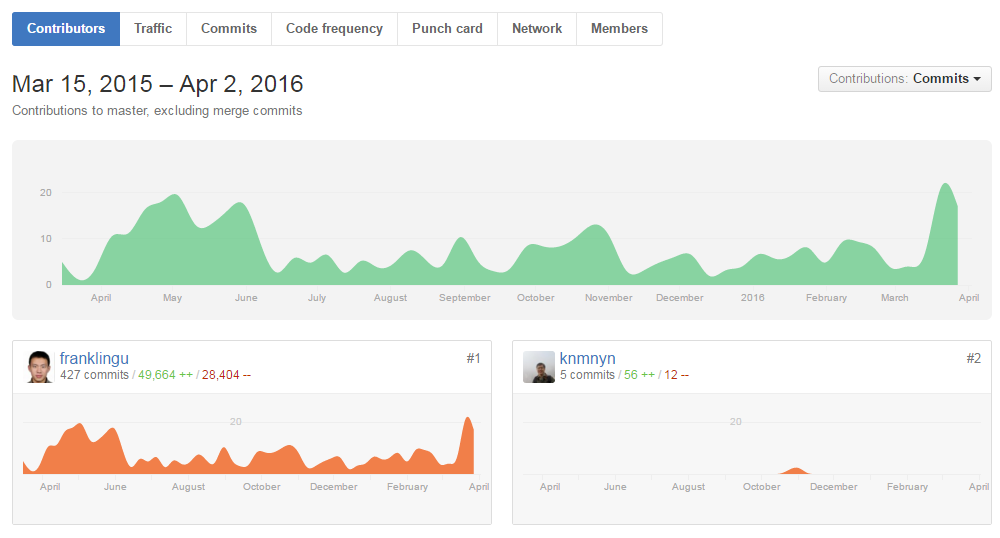
\includegraphics[width=\textwidth]{Images/Skylab_Contribution.png}
  \caption{Contribution history of Skylab}
  \label{fig:SkylabContribution}
\end{figure}

\subsection{Milestones, Deadlines and Changes}

Just like any other software engineering projects, there are many deadlines during the process. And there will always be more requirements to complete, changes to expect along the way. Throughout the entire period of implementation of Skylab, working with deadlines and changes along the way is common and this brought many practical challenges to system design as well. A timeline diagram with all important milestones is as Figure~\ref{fig:SkylabTimeline}.

\begin{figure}[h]
  \centering
  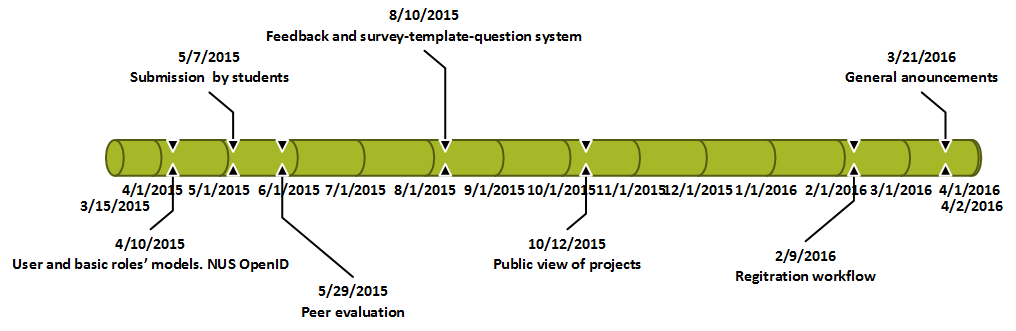
\includegraphics[width=\textwidth]{Images/Skylab_Timeline.png}
  \caption{Timeline of Skylab}
  \label{fig:SkylabTimeline}
\end{figure}

\subsection{Live Server Setup and Maintenance}

Skylab was first hosted on an Amazon EC2 instance and later migrated to an NUS SoC virtual machine. Currently, about 400 Skylab users perform their different roles.  Maintenance work is needed on the production server, necessitating a good workflow to ensure data integrity and to minimize downtime to release new versions of Skylab.

\subsection{Development Process}

We adopted the GitHub workflow for Skylab's development to facilitate agile and iterative development. Also by adopting continuous integration tool like Travis, code quality and test coverage monitoring tool like CodeClimate, security analysis tool like Hakiri, the process of ensure testing, quality and security is greatly smoothened and different issues are easily monitored.

\subsection{Major Use Cases}

Skylab is designed to serve all kinds of people involved in Orbital and it has been working to support Orbital program. From registration phase of Orbital program to last feedback in Orbital, Skylab is critical infrastructure  to the Orbital program, playing a major role in helping admins, advisers, mentors, tutors and students.

\begin{itemize}
  \item Registration: students who are interested in Orbital can sign up via Skylab. They can do this as a team of two or as individuals first. For those individuals, a match making algorithm will be run to find potential teammates based on recorded interested topics of each student.
  \item Evaluation: students and advisers will go through evaluation process in Orbital which includes submissions, peer evaluations and feedback.
  \item Administration: admins can overview things in Skylab.
  \item Mailing: various emails as reminders can be sent through Skylab.
  \item Public facing of profiles: staff of Orbital, past projects of Orbital can be displayed in Skylab easily.
\end{itemize}

\section{Future work}

While Skylab serves its purpose well, there are still limitations and enhancemens that are planned.  A proposed set of major features to be completed in the future for Skylab include:

\begin{itemize}
  \item Questions/template system (involving migration of current data): currently \textit{Feedback} and \textit{Peer Evaluation} is utilizing the \textit{SurveyTemplate} and \textit{Question} system but \textit{Submission} are still not. With a migration to the \textit{Questions} system, we can further improve the system by adding more extensibility.
  \item Logging of user activities: by logging down activities carried out by different users, administrative staff can discover problematic events and acquire situational awareness of the context in Orbital.
  \item Unit testing needs to cover more classes and acceptance testing needs to cover more use cases in Skylab, especially by different roles.
  \item Upgrade of the Rails framework to address the warnings on Hakiri and continue working on improving security.
  \item Mailing could be improved by having mailing history and other customized reminders.
\end{itemize}

